% `template.tex', a bare-bones example employing the AIAA class.
%
% For a more advanced example that makes use of several third-party
% LaTeX packages, see `advanced_example.tex', but please read the
% Known Problems section of the users manual first.
%
% Typical processing for PostScript (PS) output:
%
%  latex template
%  latex template   (repeat as needed to resolve references)
%
%  xdvi template    (onscreen draft display)
%  dvips template   (postscript)
%  gv template.ps   (onscreen display)
%  lpr template.ps  (hardcopy)
%
% With the above, only Encapsulated PostScript (EPS) images can be used.
%
% Typical processing for Portable Document Format (PDF) output:
%
%  pdflatex template
%  pdflatex template      (repeat as needed to resolve references)
%
%  acroread template.pdf  (onscreen display)
%
% If you have EPS figures, you will need to use the epstopdf script
% to convert them to PDF because PDF is a limmited subset of EPS.
% pdflatex accepts a variety of other image formats such as JPG, TIF,
% PNG, and so forth -- check the documentation for your version.
%
% If you do *not* specify suffixes when using the graphicx package's
% \includegraphics command, latex and pdflatex will automatically select
% the appropriate figure format from those available.  This allows you
% to produce PS and PDF output from the same LaTeX source file.
%
% To generate a large format (e.g., 11"x17") PostScript copy for editing
% purposes, use
%
%  dvips -x 1467 -O -0.65in,0.85in -t tabloid template
%
% For further details and support, read the Users Manual, aiaa.pdf.


% Try to reduce the number of latex support calls from people who
% don't read the included documentation.
%
\typeout{}\typeout{If latex fails to find aiaa-tc, read the README file!}
%


\documentclass[]{aiaa-tc}% insert '[draft]' option to show overfull boxes
\usepackage{amsmath}
\usepackage{graphicx}
 \title{Title}

 \author{
  Kevin Nastasi\thanks{Ph.D. Candidate, Aerospace and Ocean Engineering, and more},\ 
    Dylan Thomas\thanks{Ph.D. Candidate, Aerospace and Ocean Engineering, and more},\ 
    Kristen Tetreault\thanks{Ph.D. Candidate, Biomedical Engineering and Mechanics, and more},\\ 
    Ian Elliott\thanks{Undergraduate, Aerospace and Ocean Engineering, Address, and AIAA Member Grade.},\ 
    Robert Schieble\thanksibid{4} \ and 
    Jonathan Black \thanks{Associate Professor, Aerospace and Ocean Engineering, Address, and AIAA Member Grade.}\\
  {\normalsize\itshape
   Virginia Polytechnic Institute and State University, Blacksburg, Virginia, 24061, USA}\\
%  \and
%  Third C. Author%
%   \thanks{Job Title, Department, Address, and AIAA Member Grade.}\\
%  {\normalsize\itshape
%  Business or Academic Affiliation, City, Province, Zipcode, Country}
 }

 % Data used by 'handcarry' option if invoked
 \AIAApapernumber{YEAR-NUMBER}
 \AIAAconference{Conference Name, Date, and Location}
 \AIAAcopyright{\AIAAcopyrightD{YEAR}}

 % Define commands to assure consistent treatment throughout document
 \newcommand{\eqnref}[1]{(\ref{#1})}
 \newcommand{\class}[1]{\texttt{#1}}
 \newcommand{\package}[1]{\texttt{#1}}
 \newcommand{\file}[1]{\texttt{#1}}
 \newcommand{\BibTeX}{\textsc{Bib}\TeX}
 
 % Bibliography Packages
 \usepackage{cite}
 \usepackage{url}
 \bibliographystyle{plain}

\begin{document}

\maketitle

\begin{abstract}
\end{abstract}

\section*{Nomenclature}

\begin{tabbing}
  XXX \= \kill% this line sets tab stop
  $A$ \> State Transition Matrix \\
  $B$ \> Control Input Model \\
  $u$ \> Control Vector \\
  $P$ \> State Covariance Matrix \\
  $Q$ \> Process Noise Covariance \\
  $H$ \> Measurement Map Matrix \\
  $\Delta t$ \> Time Step, seconds \\
  $t$ \> Time, seconds \\
  $X$ \> State \\
  $I(N)$ \> Identity Matrix of size NxN
 \end{tabbing}

\section{Introduction}

\subsection{Previous Work}

\subsubsection{Background}

Setting up the scenario

\section{Model}


\subsection{ODTK}

\subsection{GVE}

\subsection{HCW}

HCW Proxops

\subsubsection{Adaptive, objective mpc}

fancy words

\subsubsection{Measurement Simulation and Filtering}

A brief study of different possible sensor systems was conducted.  Ultimately a combination of camera tracking system and a laser range-finder are used to find direction and range, respectively.  A phased-array radar system was considered, and may be explored in later research; however, the size of current systems is prohibitive.

The laser-rangefinder the MATLAB simulation uses is a FLIR MLR1001.  The data sheet cites a range from near 0 cm to over 100 m, and a resolution under 0.2 m1.  For the purposes of the MATLAB simulation, the measured range is found by taking the true range, adding a random Gaussian-distributed error with a standard deviation of 0.0255, and rounding to the closest 0.2 m increment.  The standard deviation of 0.0255 provides a 95% confidence bound of 0.1 m.

A camera tracking system would be used to find the direction of the target.  This simulation is very simplistic; the camera can track the target in all conditions, and does not simulate target acquisition.  The tracking camera is assumed to have an order of magnitude more error than the star tracker; 60 arc seconds 1-sigma bore sight accuracy, and 400 arc seconds 1-sigma roll axis accuracy.  These values are based off of the Blue Canyon Nano Star Tracker2.

A Kalman filter is used to reduce the error and estimate the position.  The equations for a Kalman filter can be found in section 3.3.1 of Crassidis and Junkins.  The state is the relative position and relative velocity.
\begin{equation}
  X = \begin{bmatrix}
    x \\
    y \\
	z \\         
    \dot{x} \\
    \dot{y} \\
    \dot{z} \\
    \end{bmatrix}
  \end{equation}
  
The state transition matrix is a simple propagation using Euler's method.  As the simulation itself propagates with Euler's method, a more robust system model causes unnecessary drift.
\begin{equation}
A = \begin{bmatrix}
1&0&0&\Delta t&0&0 \\
0&1&0&0&\Delta t&0 \\
0&0&1&0&0&\Delta t \\
0&0&0&1&0&0 \\
0&0&0&0&1&0 \\
0&0&0&0&0&1 \\
\end{bmatrix}
\end{equation}
  
  The acceleration is accounted for as a control-input u, containing both the thrust of the spacecraft and the calculated HCW accelerations.  The control-input model uses Euler’s method to update the state, so position is not affected by acceleration.
\begin{equation}
B = \begin{bmatrix}
0&0&0 \\
0&0&0 \\
0&0&0 \\
\Delta t&0&0 \\
0&\Delta t&0 \\
0&0&\Delta t \\
\end{bmatrix}
\end{equation}

\begin{equation}
u = \begin{bmatrix}
\ddot{x} \\
\ddot{y} \\
\ddot{z} \\

\end{bmatrix}
\end{equation}
  
  A Montecarlo simulation was used to find information on the performance of the Kalman filter.  The simulation output the root mean squared error of the estimated position, giving a single number to tune the filter with.  The state covariance matrix P, process covariance matrix Q, and measurement covariance matrix R, are identity matrices multiplied by a single value.  The filter was tuned by testing six possibilities for each value, ranging from 10-1 to 10-6, by order of magnitude.  This resulted in the following matrices, with a root mean squared error of 44.7854 over 2000 data points.
  
\begin{equation}
P = 10^{-4}*I(6)
\end{equation}
\begin{equation}
Q = 10^{-3}*I(3)
\end{equation}
\begin{equation}
R = 10^{-1}*I(3)
\end{equation}
  
  
\section{Results}


\subsection{odtk}

more results

\subsection{rend/proxops}

more results

\subsection{Measurement Simulation and Filtering}
The results for the position error in a Montecarlo simulation of 1000 runs can be seen in Fig:
\ref{fig:xErrorPlot},
\ref{fig:yErrorPlot}, 
\ref{fig:zErrorPlot}.  
The Kalman filter clearly reduces error across the board; however, there is an initial discrepancy in the z-position due to assuming an incorrect initial z velocity (Fig. \ref{fig:zErrorPlot}).  The maximum 95\% confidence bound for any estimate error is about 0.08 meters.  As the simulation has a safety buffer of 0.5 meters, this is well within the acceptable range.  Even without using a filter at all, the maximum measurement error is 0.1 meters, leaving a factor of safety of 5.  The filter reduces the error to about 0.02 meters for x, about 0.001 meters for y, and about 0.001 meters for z as well. 


\begin{figure}
  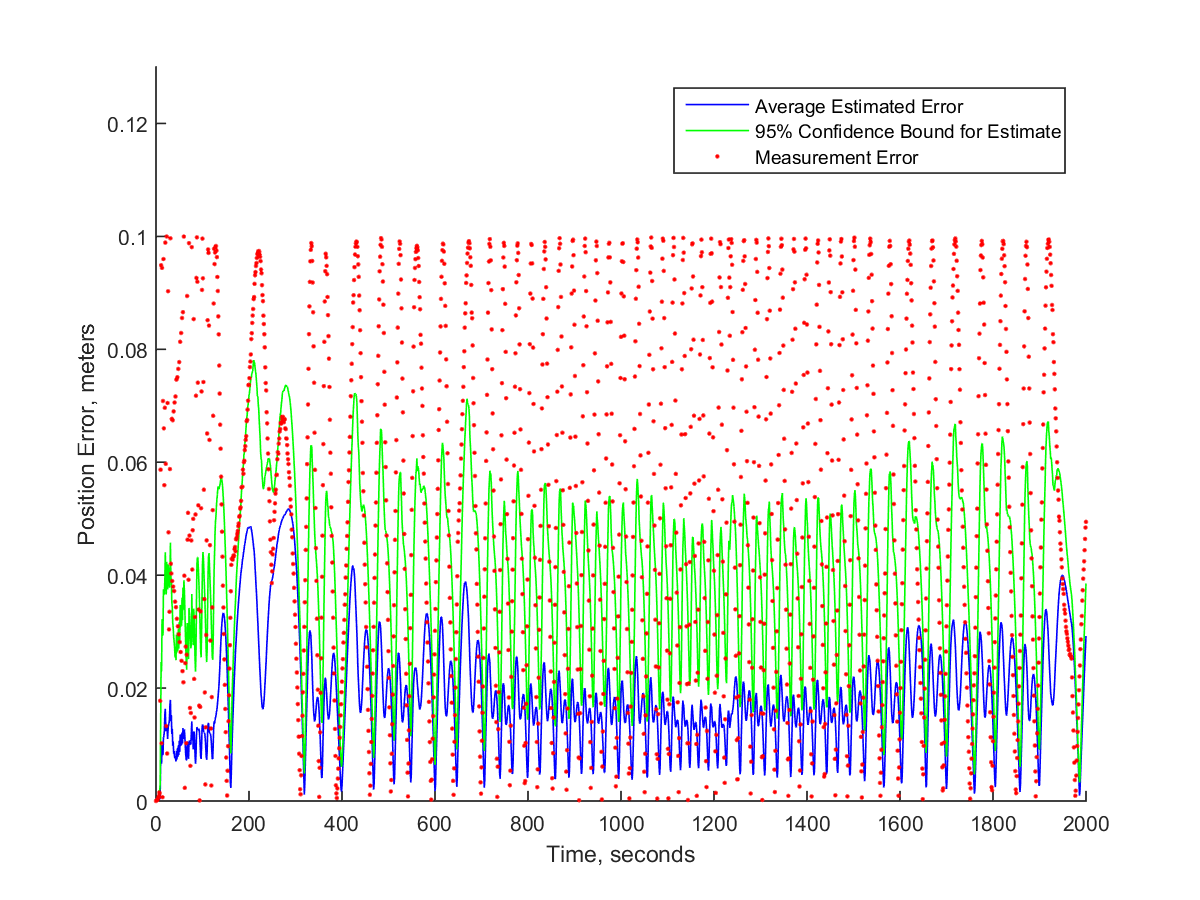
\includegraphics[width=\linewidth]{xErrorPlot.png}
  \caption{x Position Error}
  \label{fig:xErrorPlot}
\end{figure}

\begin{figure}
  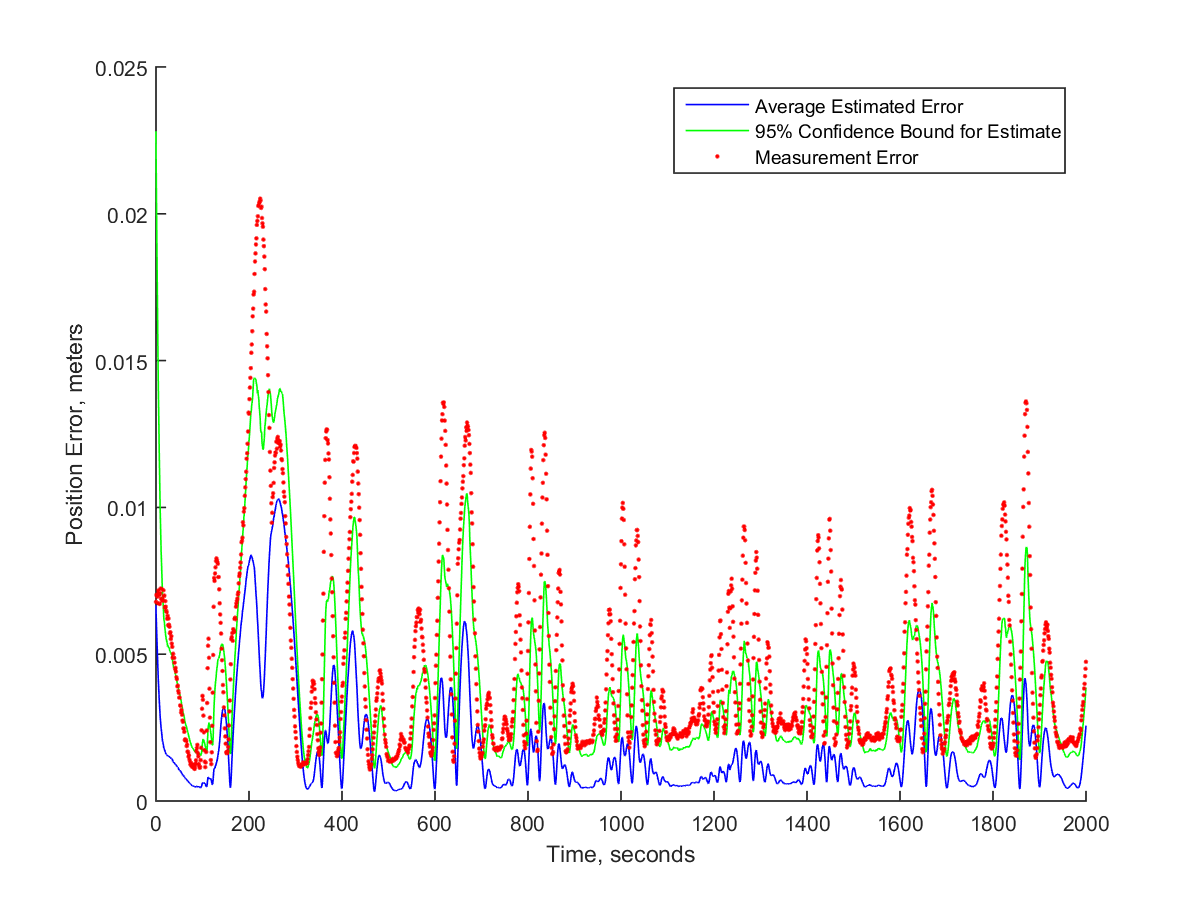
\includegraphics[width=\linewidth]{yErrorPlot.png}
  \caption{y Position Error}
  \label{fig:yErrorPlot}
\end{figure}

\begin{figure}
  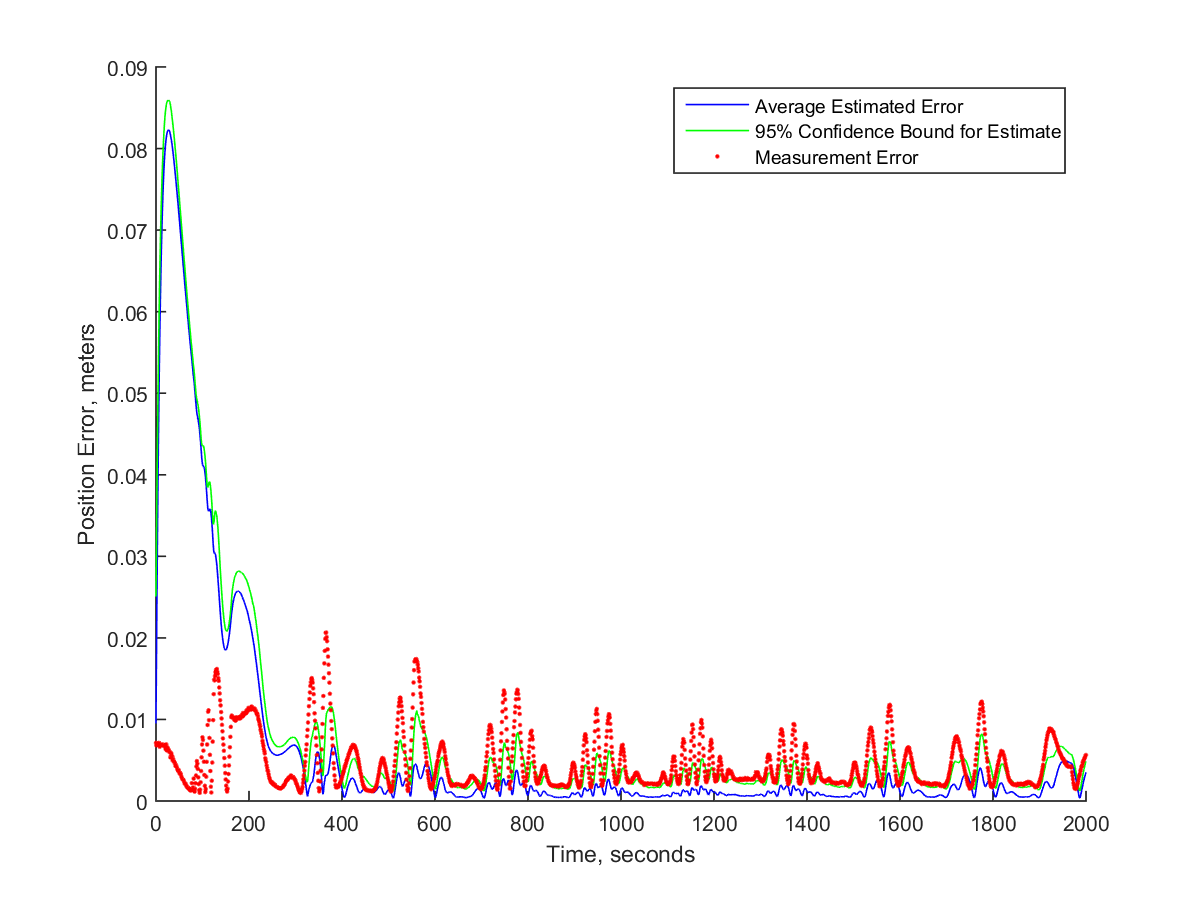
\includegraphics[width=\linewidth]{zErrorPlot.png}
  \caption{z Position Error}
  \label{fig:zErrorPlot}
\end{figure}

\section{Conclusion}

After much typing, the paper can now conclude.
Four rocks were next to the channel.
This caused a few standing waves during the rip that one could ride on
the way in or jump on the way out.

type the conclusion

\subsection{future work}

how to list this...

\subsubsection{better eoms}

adfgdsg

\subsubsection{integration of rel. od into control}

asdgadg

\subsubsection{attitude d\&c}

asdgadg

\subsubsection{cad model for more realistic 6u design}

asdgadg

\section*{Appendix}

An appendix, if needed, should appear before the acknowledgments.
Use the 'starred' version of the \verb|\section| commands to avoid
section numbering.

\section*{Acknowledgments}

A place to recognize others.

\begin{thebibliography}{9}% maximum number of references (for label width)
\bibitem{crassidis} Crassidis, John L., and Junkins, John L., “Optimal Estimation of Dynamic Systems,” 2^{nd} ed., CRC Press, New York, 2012, Chap. 3.3.1.

\end{thebibliography}

\end{document}

% - Release $Name:  $ -
